% TUTORIAL DE C
%
%
%
%
%
%
%

\documentclass[a4paper, twoside]{book}
\frenchspacing
\usepackage[spanish]{babel}
\usepackage{makeidx}
\usepackage{graphicx}
\makeindex
\pagestyle{headings}
\title{Lenguaje C}

\begin{document}
\maketitle

He empezado a escribir esto por distintas razones. La primera porque
siempre he estado buscando un libro un poco decente de aprendizaje de
alg\'un lenguaje de programaci\'on. En el mercado existen muchos, pero 
la mayor\'{\i}a creo que los conocemos todos; programaci\'on de C++,
programaci\'on de C++, programaci\'on de Visual C++, programaci\'on 
de C++, y todos por el mismo estilo; a parte de costarte el m\'as 
barato sobre unas 5.000 pesetas pasando por 7.000, 10.000, etc., cosa 
que sigo viendo abusiva no s\'olo en estos libros sino en el resto y
contando que lo \'unico que nos ofrecen son un mont\'on de p\'aginas
fotocopiadas, eso s\'{\i}, encuadernados (que algunos dejan mucho que
desear); y luego un CDROM donde la mayor parte de los archivos y 
programas son completamente in\'utiles. Luego existen por ah\'{\i} 
multitud de tutoriales que est\'an incompletos, mal redactados, 
en formato HTML y sobre todo shareware que no est\'a  completo.

En segundo lugar, creo que puedo ofrecer en lo que pueda un verdadero
libro que se pueda imprimir poco a poco seg\'un cada uno la posibilidad
que tenga y sus necesidades. El porque de este libro es simplemente la
p\'erdida de tiempo que yo he tenido buscando por la red librer\'{\i}as
y dem\'as lugares y porque creo que aprender un lenguaje como este no
deber\'{\i}a costarte 10.000 pesetas y eso s\'olo para comenzar.
Ahora existe la posibilidad de tener un compilador como es \texttt{gcc}
sin tener que pagar las absurdas cantidades que nos piden las 
compa\~n\'{\i}as por un compilador, aparte de tener que tragar con sus
librer\'{\i}as.

En tercer lugar tengo que decir que estoy en un momento en el que yo
mismo soy el que aprendo, y no s\'olo C, sino tambi\'en \LaTeX{} por
lo que habr\'a  errores de  todo tipo, ``paciencia''.

Tengo que decir que la informaci\'on de este libro en su mayor parte
est\'a recopilada de otros libros, tutoriales, etc. y de mis no muy 
grandes conocimientos, que yo he intentado
ir colocando de una forma que considero de la mejor forma para un
 principiante y que no se pierda, eso s\'{\i}, no entro en detalles
matem\'aticos tales como hexadecimales, binarios, definiciones de
bucles y todo lo relacionado con principios  de programaci\'on, que 
se podr\'an obtener de otros libros. Lo mismo puedo decir de los 
ejemplos ya que si no el libro podr\'{\i}a tener unas dimensiones 
considerablemente absurdas.

Estoy abierto a cualquier sugerencia, incluso si alguien quiere
 continuarlo porque cree que lo puede hacer mejor que yo, que no
quiere decir que lo yo lo deje. Pero esto ir\'a a la velocidad que
me pueda permitir. Tambi\'en estoy abierto a sugerencias de tipo
sint\'actico o sem\'antico debido a que hace tiempo que no leo un
libro, algo que tengo que remediar lo antes posible, y \'ultimamente
tengo un vocabulario un tanto escaso.

En un principio y como le promet\'{\i} o eso creo a un colaborador
de Linux es mandarlo lo m\'as r\'apido posible, y empezar\'e por lo
que ya tengo hecho, los dos primeros temas, sin tablas de contenido
ni \'{\i}ndices, \ldots, no hasta que est\'e un poco m\'as completo.

Para cualquier comentario, duda, inter\'es o quien sabe qu\'e, voy a
dar dos direcciones de correo, una la de un amigo que es donde sea 
m\'as sencillo encontrarme si no tiene el correo saturado o no 
vuelve a cambiar por en\'esima vez de ISP y es afios@lander.es
y la otra la que tengo en la universidad
q42derem@lucano.uco.es

Espero que pueda servir de ayuda a alguien.

\chapter{Introducci\'on al Lenguaje C}

\textsf{El objetivo de este tutorial es el aprendizaje del lenguaje C, en el que
se incluir\'{a}n problemas al final de cada cap\'{\i}tulo (que para una
mayor comprensi\'on deber\'{\i}an hacerse). Intentar\'e en lo m\'as posible
referirme al C para sistemas basados en UN*X y concretamente en Linux.}

\section{Or\'{\i}genes de C}

C es un lenguaje de prop\'osito general, control de flujo y de estructuras
de datos con un rico conjunto de operadores. C no es un \emph{lenguaje de
alto nivel} y no est\'a especializado en ning\'un \'area de aplicaci\'on 
especial.

Originalmente fue desarrollado por y como una implementaci\'on del sistema
operativo UN*X para que corriera sobre las m\'aquinas DEC PDP--11 por 
Dennis Ritchie. C no es espec\'{\i}fico de ning\'un hardware en particular 
o sistema, sin embargo, es f\'acil escribir programas que se ejecutar\'an
sin cambios en cualquier m\'aquina que soporte C, o a veces s\'olo se
tendr\'an que hacer algunos peque\~nos cambios para portarlo; se
 intentar\'a explicar los tipos de funciones y otros aspectos 
fundamentales de este tipo durante el curso del libro.

C se ha escrito para ser en lo posible los m\'as ameno, expresivo y
 vers\'atil posible  para una gran variedad de programas. Es f\'acil
\footnote{En comparaci\'on con otros, claro est\'a}
y se aprende sobre todo con la experiencia.
\footnote{Es importante entender en lo posible los
ejemplos e intentar hacer la mayor\'{i}a de los ejercicios}

Normalmente el lenguaje C se ha asociado al sistema operativo UN*X, muchas
de las ideas importantes de este provienen del lenguaje BCPL desarrollado
por Martin Richard; a su vez \'este precede indirectamente del lenguaje B, 
escrito por Ken Thompson en 1970 para el primer UN*X en la DEC PDP--7. Su
nombre es un sarcasmo de los anteriores lenguajes que se llamaron A y B.

BCPL y B son lenguajes \emph{bajo tipo}. En contraste, C suministra
una gran variedad de tipos de datos, de los cuales los fundamentales
son caracteres, enteros y n\'umeros de coma flotante de varios 
tama\~nos. Hay una jerarqu\'{\i}a de tipos de datos derivados creados 
con punteros, vectores, estructuras y uniones. Las expresiones est\'an 
formadas por operadores y operandos; cualquier expresi\'on, incluida una
asignaci\'on o una llamada a una funci\'on puede ser una declaraci\'on.
Los punteros son suministrados para la aritm\'etica de direcciones 
independientemente de la m\'aquina. M\'as tarde, debido al surgimiento
de distintas variedades de C se defini\'o un est\'andar que hoy en 
d\'{\i}a est\'a representado por el ANSI C.

C suministra las construcciones elementales para un control de flujo 
requerido para una buena estructuraci\'on de los programas: agrupaci\'on de
declaraciones, toma de decisiones (\texttt{if-else}), selecci\'on de 
posibles casos (\texttt{switch}), lazos (\texttt{while, for, do}) y salida
de estos (\texttt{break}). 

Las funciones pueden devolver valores de tipos b\'asicos, estructuras, uniones
 o punteros. Las variables locales normalmente son \emph{autom\'aticas}.
La definici\'on de las funciones puede que no est\'en anidadas pero las
variables se pueden declarar en bloques estructurados. Las funciones pueden
existir en distintos ficheros que se compilar\'an por separado. Las variables 
pueden ser internas a la funci\'on o externas,  reconocidas
dentro del propio fichero o visibles para todo el programa.

Los preprocesos son macro sustituciones en programas de texto que incluyen 
otros ficheros fuente y una compilaci\'on condicional.

C relativamente es un lenguaje de \emph{bajo nivel}, pero esto es una 
definici\'on un tanto ambigua, significa que C trata con el mismo orden
los objetos tal como la mayor\'{\i}a de las computadoras, nombrando
caracteres, n\'umeros y direcciones. Esto puede ser combinado y transladado
con los operadores aritm\'eticos y l\'ogicos implantados en m\'aquinas
reales.

C no trata a las operaciones directamente con una composici\'on de objetos
como cadenas de caracteres, conjuntos, listas o vectores; no hay operaciones
que manipulen cadenas o vectores por completo, aunque las estructuras se
pueden copiar como unidades. Por \'ultimo no suministra facilidades de E/S, no
\footnote{entrada/salida o I/O del ingl\'es input/output}
existen declaraciones como READ o WRITE \footnote{LECTURA o ESCRITURA} y 
ninguna construcci\'on de acceso a ficheros. Esto se hace mediante llamadas
a funciones.

Con todo esto dicho hasta ahora vamos a comenzar con una introducci\'on 
de las bases del lenguaje que se desarrollar\'an con mayor amplitud en 
cap\'{\i}tulos posteriores. As\'{\i} daremos algunas nociones sobre distintos
conceptos y definiciones para que se familiarice con el lenguaje sin entrar
en detalles.

\section{Uso de C}

Los pasos que hay que seguir desde que se empieza a escribir un programa
hasta que se ejecuta son los siguientes:

\begin{itemize}
\item \textbf{Escribirlo:} El programa se tiene que escribir en un editor 
de testos est\'andar que no genere c\'odigos de control o caracteres no 
imprimibles (puedes elegir una gran variedad tales como emacs, vi, ed, etc. \
). Los ficheros fuente son aquellos que contiene el c\'odigo fuente que 
ser\'an leidos por el compilador. Si son peque\~nos ocupar\'an un fichero,
pero a medida que crecen ser\'a necesario distribuirlo en m\'as de uno. Los
ficheros tiene que acabar con la extensi\'on en \texttt{.c}.

\item \textbf{Compilarlo:} El compilador produce ficheros objeto, que contienen
c\'odigo objeto, e.d., ficheros con c\'odigo m\'aquina y que son utilizados
como entrada  al enlazador. En el caso de Linux se producen cuando la 
compilac\'on se realiza para m\'as de un fichero.
La forma de compilarlo es con el comando 
\texttt{cc}, \texttt{gcc} o con el \'ultimo compilador que se ha desarrollado
para Linux \texttt{egcs}. En el caso de un \'unico
fichero dar\'a como resultado un fichero ejecutable llamado \texttt{a.out}.
La extensi\'on de los ficheros objeto es \texttt{.o}.

\item \textbf{Enlazarlo:} El enlazador produce un fichero ejecutable a 
partir de los ficheros objeto. Los ficheros ejecutables contienen c\'odigo
m\'aquina y se pueden ejecutar directamente por el sistema operativo. La
palabra inglesa que da origen a la denominaci\'on de enlace es \emph{link}.

\item \textbf{Ejecutarlo:} El programa se puede ejecutar directamente
ejecutando su nombre (\texttt{./a.out}) en la l\'{\i}nea de comandos.

\end{itemize}

\section{Primeros Pasos}

La mejor forma de aprender C, como la mayor\'{\i}a de los lenguajes es 
escribir programas desde un principio para tener una noci\'on de estos
y una mayor comprensi\'on. ?`Y por que no?, empezaremos con el ejemplo
m\'as t\'{\i}pico de todos. La impresi\'on del texto \emph{hola, mundo}.

\begin{quotation}
\begin{verbatim}

#include <stdio.h>

main()
{
   printf("hola, mundo\n");
}

\end{verbatim}
\end{quotation}

Para ejecutar este programa ejecutamos el 
comando  \texttt{gcc fichero.c}. Si 
todo est\'a bien, se producir \'a la compilaci\'on
y dar\'a lugar a  un fichero ejecutable llamado
 \texttt{a.out}, que si lo ejecutas produce la salida

\begin{quotation}
\begin{verbatim}

hola, mundo

\end{verbatim}
\end{quotation}

en otros sistemas las reglas pueden ser diferentes, pero normalmente
en Linux es de esta manera.

Ahora vamos a explicar el programa. Un programa en C consiste en \emph{funciones}
y \emph{variables}. Una funci\'on contiene \emph{declaraciones} que especifican 
la forma en que se har\'a la computaci\'on. En el ejemplo, la funci\'on se 
llama \texttt{main}
\index{main} 
(principal) y es una funci\'on especial--el programa 
comienza ejecut\'andose
al principio de  \texttt{main}, lo que significa que cada programa tiene que tener 
una funci\'on  \texttt{main} en alg\'un lugar. Esta funci\'on normalmente llama a 
otras funciones para aydar a ejecutar su trabajo, de lo que has escrito y de las 
librer\'{\i}as que se te suministran.


Las funciones pueden comunicar datos suministrando una lista de valores que va entre 
par\'entesis, estos son llamados \emph{argumentos} hacia la funci\'on llamada. En 
este ejemplo la funci\'on no tiene argumentos, esto se indica con los par\'entesis
vac\'{\i}os.


La primera l\'{\i}nea del programa

\begin{quotation}
\begin{verbatim}

#include <stdio.h>

\end{verbatim}
\end{quotation}

\index{include}

le dice al compilador que incluya informaci\'on sobre la librer\'{\i}a de E/S
est\'andar; esta l\'{\i}nea aparece al comienzo de la mayor parte de los
 programas de C. Una l\'{\i}nea que comienza con \# en realidad no es una 
instrucci\'on del lenguaje C, sino que son l\'{\i}neas que se manipulan 
por el preprocesador. El preprocesador realiza algunas tareas antes de 
empezar a actuar con el compilador. Esta l\'{\i}nea incluye la informaci\'on 
que hay en el fichero \texttt{stdio.h} en el programa, en este fichero se 
encuentra la definci\'on de la  funci\'on \texttt{printf}. Si no 
pusi\'eramos este \texttt{include} en el programa el compilador nos 
dar\'{\i}a un error al no saber como es la funci\'on \texttt{printf}.


Las declaraciones de una funci\'on est\'an encerradas entre 
llaves \{ \}. La funci\'on \texttt{main} contiene una sola declaraci\'on,

\begin{quotation}
\begin{verbatim}

printf("hola, mundo\n");

\end{verbatim}
\end{quotation}

\index{printf}

A una funci\'on se la llama nombr\'andola, seguida por unos par\'entesis entre los 
que hay una lista de argumentos. Esta funci\'on imprime la salida, que en este caso
es una \emph{cadena de caracteres}, se llama  as\'{\i} a los caracteres que van entre
comillas dentro de la funci\'on.


En la cadena hay una secuencia al final de la forma 
\texttt{$\backslash$n}, a estos caracteres se
 les llama \emph{secuencias de 
escape} y en este caso  es la notaci\'on en C es el car\'acter de
\emph{car\'acter de nueva l\'{\i}nea}, avanza la salida al margen izquierdo en 
la siguiente l\'{\i}nea. Si no se coloca no habr\'a avance de l\'{\i}nea a la salida
del programa. Este ejemplo se podr\'{\i}a haber escrito como


\begin{quotation}
\begin{verbatim}

#include <stdio.h>

main()
{
   printf("hola,");
   printf("mundo");
   printf("\n");
}



\end{verbatim}
\end{quotation}

dando el mismo resultado, debido al caracter de nueva l\'{\i}nea que no se encuentra
hasta la \'ultima funci\'on \texttt{printf}. Adem\'as de este car\'acter hay otros que
se explicar\'an en otro momento.

\section{Variables y Expresiones Aritm\'eticas}

El siguiente programa usa la f\'ormula C = (5/9)(F-32) para imprimir una tabla 1 de conversi\'on 
de temperaturas entre Fahrenheit y Celsius.

\begin{quotation}
\begin{verbatim}

0      -17
20     -6
40     4
60     15
80     26
100    37
120    48
140    60
160    71
180    82
200    93
220    104
240    115
260    126
280    137
300    148


\end{verbatim}
\end{quotation}

Ahora vemos el programa que produce esta salida, el cual s\'olo lleva una funci\'on, que es 
\texttt{main}, la misma que en el anterior. Aqu\'{\i} introducimos nuevas ideas
como comentarios, declaraciones, variables, expresiones aritm\'eticas, lazos y salida
formateada.

\begin{quotation}
\begin{verbatim}

#include <stdio.h>

/*impresion de una tabla Fahrenheit-Celsius
   para farh = 0, 20, ..., 300 */
main()
{
   int fahr, celsius;
   int inferior, superior, paso;
   
   inferior = 0;     /*limite mas bajo en tabla*/
   superior = 300;   /*limite superior*/
   paso = 20;        /*tamano del paso*/
   
   fahr = inferior;
   while (fahr <= superior) {
      celsius = 5 * (fahr-32) / 9;
      printf("%d\t%d\n", fahr, celsius);
      fahr = fahr + paso;
   }
}

\end{verbatim}
\end{quotation}

Las dos l\'{\i}neas

\begin{quotation}
\begin{verbatim}

/*impresi�n de una tabla Fahrenheit-Celsius
   para farh = 0, 20, ..., 300 */

\end{verbatim}
\end{quotation}

son \emph{comentarios}. Cualquier car\'ater que est\'e encerrado entre
los s\'{\i}mbolos \texttt{/*} y \texttt{*/} es ignorado por el compilador;
se recurre a ellos para dar detalles sobre cualquier operaci\'on llevada 
a cabo en el programa, haci\'endolo m\'as legible por el lector. Los 
comentarios pueden aparecer en cualquier lugar.

En C, todas las variables \emph{tienen que declararse antes de ser usadas},
normalmente se hace al principio de la funci\'on, antes de cualquier declaraci\'on
ejecutable. Una \emph{declaraci\'on} nos comunica las propiedades de las 
variables, consiste en un tipo de variable y una lista de variables como en

\begin{quotation}
\begin{verbatim}

int fahr, celsius;
int inferior, superior, paso;

\end{verbatim}
\end{quotation}

El tipo \texttt{int} significa que las variables que vienen a continuaci\'on
son enteras, otro tipo ser\'{\i}a {texttt{float}, que es un n\'umero en 
coma flotante, e.d., un n\'umero con parte fraccionaria. Sobre los tipos 
de variables y sus longitudes se comentar\'a en el siguiente cap\'{\i}tulo.
Las variables son posiciones en memoria donde el valor de su contenido
puede variar a lo largo del programa.

De momento diremos que el tama\~no de los objetos es dependiente del tipo
de m\'aquina, lo que podr\'{\i}a hacerlo no portable.

La computaci\'on en el programa de conversi\'on de temperaturas comienza
con las \emph{sentencias de asignaci\'on}

\begin{quotation}
\begin{verbatim}

inferior = 0;
superior = 300;
paso = 20;
fahr = inferior;

\end{verbatim}
\end{quotation}

que pone a las variables sus valores iniciales. Las declaraciones individuales
terminan con un punto y coma ``\texttt{;}''.

Cada l\'{\i}nea del programa es computado de la misma forma,  usamos un lazo
que repite una por una las l\'{\i}neas de salida

\begin{quotation}
\begin{verbatim}

while (fahr <= superior) {
    ...
}

\end{verbatim}
\end{quotation}

\index{while}

El lazo \texttt{while} opera de la siguiente manera: La condici\'on entre 
par\'entesis es evaluada, si es cierta (\texttt{fahr} es menor o igual que
\texttt{superior}), el cuerpo del lazo (las tres declaraciones encerradas 
entre llaves) se ejecuta. Luego la condici\'on es reevaluada y si es cierta
se vuelve a ejecutar. Cuando el la condici\'on es falsa, el lazo termina y
la ejecuci\'on contin\'ua con la siguiente declaraci\'on que sigue al lazo.
En este programa no hay m\'as declaraciones, por lo que termina.
El cuerpo del un lazo \texttt{while} puede tener una o m\'as declaraciones 
encerradas entre llaves.

En este momento vamos a hacer una peque\~na sugerencia para el lector, y es que
es importante seguir unas pautas en la construcci\'on de un programa, e.d.,
que debemos utilizar una determinada tipograf\'{\i}a. Normalmente existen
programas en los que se puede editar un programa y ellos mismos van creando
una forma de situar cada l\'{\i}nea para hacerlo lo m\'as legible posible tal
como \texttt{jed}, \texttt{xwpe}, \ldots en Linux. Lo mejor es elegir una
forma, la que m\'as te guste y mantenerla.

Pasamos a la siguiente l\'{\i}nea

\begin{quotation}
\begin{verbatim}

celsius = 5 * (fahr-32) / 9;

\end{verbatim}
\end{quotation}

como a primera vista parece es simplemente la definici\'on de una funci\'on que
se computar\'a y nos dar\'a unos resultados; es de forma aproximada la 
f\'ormula de conversi\'on de temperatura entre Fahrenheit y Celsius. Una cosa
que en  un primer momento llama la atenci\'on es que primero se multiplica por
5 y despu\'es al final se divide por 9, en lugar de multiplicar directamente
por 5/9. Esto es porque en C, como en otros lenguajes, la divisi\'on de enteros
est\'a truncada: cualquier parte fraccionada es descartada. Al ser 5 y 9 dos
enteros, 5/9 nos dar\'{\i}a como resultado 0 y la conversi\'on de todas las 
temperaturas ser\'{\i}a cero.

Este ejemplo tambi\'en nos muestra algo m\'as de la funci\'on \texttt{printf},
esta es una funci\'on de prop\'osito general que nos da la salida de una 
funci\'on formateada, que se describir\'a con m\'as detalle en posteriores
cap\'{\i}tulos. Su primer argumento ya es conocido por el programa anterior,
se trata de una cadena de caracteres que ser\'an impresos en este caso por 
pantalla. Pero entre ellos hay unos caracteres distintos en un principio a 
todos los dem\'as, que son dos s\'{\i}mbolos de la forma \texttt{\%d}.
Su prop\'osito es provocar la salida de las variables que siguen a 
continuaci\'on despu\'es de las comillas, e.d., el valor que tendr\'an en este
paso. as\'{\i} el primer  \texttt{\%d} corresponde a la variable \texttt{fahr}
y el segundo a la variable \texttt{celsius}. Estos argumentos son del tipo
entero (por que lo que los sigue es una \texttt{d}), pero hay otros como
 \texttt{\%f},  \texttt{\%c}, que corresponde a coma flotante y tipo 
car\'acter respectivamente. M\'as tarde en el siguiente cap\'{\i}tulo se 
comentar\'an con m\'as amplitud.

En este programa nos encontramos con algunos problemas. El primero es que la
salida no es muy vistosa y podr\'{\i}a estar mejor formateada como por ejemplo,
alineada a la derecha. Esto se puede mejorar f\'acilmente con m\'as argumentos
sobre \texttt{\%d}. Se podr\'{\i}a hacer

\begin{quotation}
\begin{verbatim}

printf(``%d3d %6d\n'', fahr, celsius);

\end{verbatim}
\end{quotation}

que imprime los primeros n\'umeros de cada l\'{\i}nea en un campo de amplitud 
de tres d\'{\i}gitos y los segundos en un campo de seis d\'{\i}gitos, tal como

\begin{quotation}
\begin{verbatim}

  0   -17
 20    -6
 40     4
 60    15
 80    26
100    37
...

\end{verbatim}
\end{quotation}

El siguiente problema es que hemos usado aritm\'etica de enteros, y las
temperaturas Celsius no est\'an ajustadas; por ejemplo,  0  grados  F 
ser\'{\i}an -17.8  grados
 C y no -17. Para solucionar este problema utilizamos la aritm\'etica
de coma flotante en lugar de los enteros. Esto requiere algunos cambios 
en el programa. Vemos una segunda versi\'on:

\begin{quotation}
\begin{verbatim}

#include <stdio.h>

/*impresi�n de una tabla Fahrenheit-Celsius
   para farh = 0, 20, ..., 300, versi�n de float */
main()
{
   float fahr, celsius;
   int inferior, superior, paso;
   
   inferior = 0;     /*limite m�s bajo de la tabla de temperatura*/
   superior = 300;   /*limite superior*/
   paso = 20;        /*tama�o del paso*/
   
   fahr = inferior;
   while (fahr <= superior) {
      celsius = (5.0/9.0) * (fahr-32.0);
      printf("%3.0f %6.1f\n", fahr, celsius);
      fahr = fahr + paso;
   }
}

\end{verbatim}
\end{quotation}

Aqu\'{\i} \texttt{fahr} y \texttt{celsius} son declaradas como \texttt{float}, 
y la f\'ormula se escribe de una manera m\'as natural. No se va a usar la forma
5/9 porque puede dar una divisi\'on de enteros dando lugar al valor de cero.
Un punto decimal en una constante indica que es coma flotante por lo que
5.0/9.0 no es truncado debido a que es el resultado de dos valores fraccionarios.

Si un operador aritm\'etico tiene operandos enteros, entonces se ejecuta una
operaci\'on de enteros; si tiene un operando de coma flotante y otro entero, este
\'ultimo se transforma en coma flotante antes de la ejecuci\'on de la operaci\'on.
as\'{\i} al escribir \texttt{(fahr-32)}, el 32 autom\'aticamente se convierte
en coma flotante. Esto se cubrir\'a en el siguiente cap\'{\i}tulo.

La especificaci\'on de conversi\'on \texttt{\%3.0f} en \texttt{printf} nos dice 
que un n\'umero de coma flotante ser\'a imprimido con al menos tres caracteres 
de amplitud, sin parte fraccionaria y sin punto decimal. \texttt{\%6.1f} describe
otro n\'umero que se imprime con al menos seis d\'{\i}gitos, con un d\\'{\i}gito
despu\'es del punto decimal. La salida de este programa es:

\begin{quotation}
\begin{verbatim}

  0   -17.8
 20    -6.7
 40     4.4
...

\end{verbatim}
\end{quotation}

Entre otros, \texttt{printf} reconoce \texttt{\%o} para octal, \texttt{\%x} para 
hexadecimal, \texttt{\%c} para car\'acter y otros que se describen en el siguiente
cap\'{\i}tulo.

\begin{itemize}

\item \textbf{Ejercicio 1}. Modifica el programa de temperaturas para que imprima
una cabecera encima de la tabla.

\item \textbf{Ejercicio 2}. Escribe un programa que imprima la tabla correspondiente
de transformaci\'on de Celsius en Fahrenheit.

\end{itemize}

\chapter{Tipos, Operadores y Expresiones}

\begin{textsf}
En esta lecci\'on se va a hacer un estudio completo sobre los tipos,
operadores y expresiones del lenguaje C. Vamos a dar unas definiciones que
se utilizar\'an a lo largo de este cap\'{\i}tulo:

\begin{itemize}

\item Las variables y constantes son los objetos b\'asicos que se manipulan en
un programa.

\item Las declaraciones indican las variables que se van a usa, su tipo y en
algunos casos su valor inicial.

\item Los operadores especifican lo que se va a hacer con las variables.

\item Las expresiones combinan variables y constantes para producir nuevos
valores.

\end{itemize}

\end{textsf}

\section{Datos}

Los programas funcionan con datos y estos son n\'umeros y caracteres que 
contienen la informaci\'on que se pretende utilizar. Hay que tener en cuenta
algunas restricciones a la hora de nombrar a las variables y las constantes
simb\'olicas. Los nombres de estas pueden ser letras y d\'{\i}gitos, aunque
el primer car\'acter siempre debe ser una letra. El subrayado ``\_'' se 
considera como una letra, pero no es aconsejable utilizarlo como primer
car\'acter de una variable. En C existe la distinci\'on entre may\'usculas y
min\'usculas por lo que es sensitivo a los caracteres (no es lo mismo 
\texttt{printf} que \texttt{Printf}). Normalmente se utilizan las min\'usculas
para darle nombre a las variables y las may\'usculas para nombrar a las 
constantes simb\'olicas. De estas \'ultimas se hablar\'a m\'as tarde.

Al menos los primeros 31 caracteres de un nombre interno son significativos.
Para los nombres de funci\'on y variables externas. el n\'umero puede que sea
menor de 31, porque los nombres de variables externas se pueden usar en
ensambladores y cargadores sobre los que no tiene control el lenguaje. Para 
estas el est\'andar s\'olo garantiza los primeros 6 caracteres.

Las palabras como \texttt{if}, \texttt{else}, \texttt{int}, \texttt{float}, 
etc., est\'an reservadas y no se pueden usar como nombres de variables.
Se aconseja que se nombren a las variables con t\'erminos relativos al
uso que les vayamos a dar  para evitar confusiones y hacer el programa
m\'as legigle, no solamente para el programador, sino tambi\'en para el lector.

Podemos hacer dos divisiones del tipo de datos donde una ser\'{\i}a respecto
a constantes y variables. Las constantes son datos con valores fijos que
no se pueden alterar por el programa y las variables son datos cuyo valor se
puede cambiar a lo largo del programa. La segunda divisi\'on corresponde a 
al tipo de estos datos. Existen cinco tipos b\'asicos en C que se describen
en la tabla 2.1.

\begin{table}[!hbp]
\begin{tabular}{|c|p{1in}|p{0.5in}|p{1.5in}|} \hline
\em Tipo & \em Descripci\'on & \em Longitud en bytes & \em Rango \\ \hline
\hline 
char & car\'acter & 1 & 0 a 255\\ \hline
int & entero & 2 & -32768 a 32767\\ \hline
float & coma flotante & 4 & aprox. 6 d\'{\i}gitos de precisi\'on\\ \hline
double & coma flotante de doble precisi\'on & 8 & aprox. 12 d\'{\i}gitos
de precisi\'on\\ \hline
void & sin valor & 0 & sin valor\\ \hline
\end{tabular}
\caption{Tipos de Datos}
\end{table}

\begin{description}

\item NOTA: La longitud como se ha dicho antes y por consiguiente el
rango, dependen
de cada tipo de procesador y del compilador de C, no obstante, esta tabla es
correcta para la mayor\'{\i}a  de computadoras.
\end{description}

Ahora vamos a dedicar un tiempo a una descripci\'on detallada de los tipos de 
datos.

\subsection{Tipo Car\'acter}

\index{char}

En C los caracteres se definen mediante ap\'ostrofos. Como ejemplos tenemos
\texttt{'T'}, \texttt{'l'}, \texttt{'1'}. Ser\'{\i}an incorrectos tipos de 
caracteres tales como \texttt{'TT'}, \texttt{l} o \texttt{1}. \texttt{'TT'} es
incorrecto porque hay dos caracteres entre los ap\'ostrofos; \texttt{l} debido 
a que el compilador lo interpreta como una variable y \texttt{1} como un 
n\'umero. El valor de una constante car\'acter es el valor num\'erico del 
car\'acter  en el conjunto de caracteres del sistema. Por ejemplo, en ASCII,
el car\'acter cero o \texttt{'0'} es 48 y en EBCDIC es 240, que son
 completamente distintos del valor num\'erico 0. Siempre que no se indique lo
contrario se usar\'a el c\'odigo ASCII. Ejemplos de asignaci\'on de este tipo
de datos.

\begin{quotation}
\begin{verbatim}

char ch1, ch2;  /*declaracion de las variables ch1 y ch2*/
ch1 = 'A';      /*a ch1 se le asigna el codigo ASCII 'A': 65*/
ch2 = 65;       /*a ch2 se le asigna el codigo 65 que es 'A'*/

\end{verbatim}
\end{quotation}

Las dos asignaciones anteriores son equivalentes, pero es preferible la
primera porque es m\'as \emph{portable}. A \texttt{ch1} en cualquier
ordenador se le asigna el car\'acter A, sin embargo, en la segunda variable
si existe otro c\'odigo se le puede asignar otro car\'acter distinto. Todas
las variables de C tienen que declararse antes de poder ser usadas. La forma
de hacerlo es:

\begin{quotation}
\begin{verbatim}

tipo variables;

\end{verbatim}
\end{quotation}

Donde \texttt{variables} es uno o m\'as nombres de identificadores separados
por comas. Las declaraciones deben estar antes de la primera sentencia
ejecutable. Como ejemplo

\begin{quotation}
\begin{verbatim}

int a, b, c;
char caracter;

\end{verbatim}
\end{quotation}

Hay ciertos caracteres no imprimibles que  se representan como constantes
de car\'acter mediante secuencias de escape. En la tabla 2.2 se muestran las
secuencias de escape del ANSI C.

\begin{table}[!hbp]
\begin{tabular}{|c|l|}
\hline
\em C\'odigo & \em Significado\\ \hline
\hline
$\backslash$a & alerta (bell, campanilla)\\ \hline
$\backslash$b & retroceso\\ \hline
$\backslash$f & salto de p\'agina\\ \hline
$\backslash$n & nueva l\'{\i}nea\\ \hline
$\backslash$r & retorno de carro\\ \hline
$\backslash$t & tabulaci\'on horizontal\\ \hline
$\backslash$v & tabulaci\'on vertical\\ \hline
$\backslash$$\backslash$ & barra invertida\\ \hline
$\backslash$0 & car\'acter nulo\\ \hline
$\backslash$'' & comillas dobles\\ \hline
$\backslash$' & comilla simple\\ \hline
$\backslash$? & marca de pregunta\\ \hline
$\backslash$ooo & n\'umero octal\\ \hline
$\backslash$xhh & n\'umero hexadecimal \\ \hline
\end{tabular}
\caption{Secuencias de Escape}
\end{table}

El car\'acter constante '$\backslash$0' representa al valor cero, el
 car\'acter nulo. No es la cifra 0, que en ASCII es 48, sino un car\'acter
no imprimible, cuyo c\'odigo en ASCII es 0.

\subsection{Tipo Entero}

\index{int}

Es un n\'umero sin parte fraccionaria. Se escribe de la forma \texttt{int 
variable}. Las constantes enteras se pueden 
escribir de tres formas distintas:

\begin{enumerate}

\item En decimal: escribiendo el n\'umero sin empezar por cero (sin contar
con el propio cero). Ejemplos: 1, 0, -2.

\item En hexadecimal: empezando por el n\'umero 0x: Ejemplos: 0xE, 0x1A, 0x4.

\item En octal: empezando el n\'umero por cero. Ejemplos: 02, 021, 050.

\end{enumerate}

\subsection{Tipos Float y Double}

\index{float}
\index{double}

Las constantes de este tipo tienen una parte real y otra fraccionaria. El tipo
\texttt{double} es igual al \texttt{float} excepto que tiene doble precisi\'on.
La sint\'axis para estos tipos es:

\begin{quotation}
\begin{verbatim}

[signo] [digitos] [.] [digitos] [exponente [signo] digitos]

\end{verbatim}
\end{quotation}

donde

\begin{quotation}

signo es + o -
digitos es una secuencia de d\'{\i}gitos
. es el punto decimal
exponente es e o E

\end{quotation}

Los elementos entre corchetes son opcionales, pero el n\'umero no puede
empezar por e o E, ya que el compilador lo interpretar\'{\i}a como un 
identificador en lugar de un n\'umero. Ejemplos: 2.3e2, 21.45, -2E-3.

\subsection{Tipo Void}

\index{void}

Significa sin valor. Uno de los usos de este tipo lo podemos ver en un ejemplo.

\begin{quotation}
\begin{verbatim}

#include <stdio.h>
void main(void)
{
   printf("ejemplo tipo void\n");
}

\end{verbatim}
\end{quotation}

Al colocar \texttt{void} entre los par\'entesis de la funci\'on, se define a 
\'esta como una funci\'on que no tiene argumentos. No confuncir con llamada a 
funci\'on, en cuyo caso \emph{no se puede utilizar} el \texttt{void}. Del mismo
modo, al poner el \texttt{void} delante de la funci\'on, se est\'a declarando
como funci\'on que no devuelve nada. Esta versi\'on ser\'a la que se 
utilizar\'a de forma preferente.

\section{Modificadores}

A excepci\'on del tipo \texttt{void}, los tipo de datos b\'asicos pueden tener
varios modificadores precedi\'endolos. Hay dos tipos de modificadores, los de
tipo y los de acceso.

\subsection{Modificadores de Tipo}

Se utilizan para alternar el significado del tipo base para que se ajuste a 
las necesidades de cada momento. Vemos los tipos en la tabla 2.3.

\index{signed}
\index{unsigned}
\index{long}
\index{short}

\begin{table}[!hbp]
\begin{tabular}{|c|c|p{2in}|} \hline
\em Modificador & \em Descripci\'on & \em Tipos a los que se les puede aplicar\\ \hline
signed & con signo & int, char\\ \hline
unsigned & sin signo & int, char\\\hline
long & largo & int, char, double\\\hline
short & corto & int, char\\ \hline
\end{tabular}
\caption{Modificadores de tipo}
\end{table}

El uso de \texttt{signed} con enteros es redundante aunque est\'a permitida, ya
que  la declaraci\'on impl\'{\i}cita asume un n\'umero con signo. En la tabla
2.4 vemos la longitud y el rango de los tipos con sus modificadores asociados.

\begin{table}[!hbp]
\begin{tabular}{|l|p{0.5in}|p{1in}|} \hline
\em Tipo & \em Longitud en bytes & \em Rango\\\hline
\hline
char & 1 & Caracteres ASCII\\\hline
unsigned char & 1 & 0 a 255\\\hline
signed char & 1 & -128 a 127\\\hline
int & 2 & -32768 a 32767\\\hline
unsigned int & 2 & 0 a 65535\\\hline
signed int & 2 & igual que int\\\hline
short int & 1 & -128 a 127\\\hline
unsigned short int & 1 & 0 a 255\\\hline
signed short int & 1 & igual que short int\\\hline
long int & 4 & -2147483648 a 2147483649\\\hline
signed long int & 4 & igual que long int\\\hline
unsigned long int & 4 & 0 a 4294967296\\\hline
float & 4 & aprox. 6 d\'{\i}gitos de precisi\'on\\\hline
double & 8 & aprox. 12 d\'{\i}gitos de precisi\'on\\\hline
long double & 16 & aprox. 24 d\'{\i}gitos de precisi\'on\\\hline
\end{tabular}
\caption{Descripci\'on de los distintos tipos}
\end{table}

\subsection{Modificadores de Acceso}

\index{const}
\index{volatile}

Como su nombre indica, modifican el acceso a los tipos y hay dos tipos: 
\texttt{const} (constante) y \texttt{volatile} (vol\'atil). Las variables de
tipo \texttt{const} son aquellas a las que se les asigna un valor inicial y no
puede cambiarse a lo largo del programa. Se utilizan para declarar constantes.
Las variables de tipo \texttt{volatile} previenen al compilador de que esta
 variable se puede cambiar por medios no expl\'{\i}citamente especificados
por el programa. Por ejemplo:

\begin{quotation}
\begin{verbatim}

int a;
a = 1;
a = 2;

\end{verbatim}
\end{quotation}

En estos casos el compilador suele optimizar el c\'odigo y la primera sentencia
se deshecha y no se genera c\'odigo para ella ya que es redundante. Si la 
hubi\'esemos declarado como ``\texttt{volatile v}'', la optimizaci\'on no se
 realiza sobre la variable $a$, \emph{gener\'andose c\'odigo para las dos
asignaciones}.

En C tambi\'en existen \emph{tipos derivados}, que como su nombre indica 
derivan de los tipos b\'asicos. Vamos a ver un tipo b\'asico muy com\'un en
C: las \emph{cadenas de caracteres}.

\section{Cadenas de Caracteres}

\index{cadena de caracteres}

Una cadena de caracteres es una secuencia de caracteres encerrados entre
comillas. Por ejemplo:

\begin{quotation}
\begin{verbatim}

"Esto es una cadena de caracteres"
"abc"

\end{verbatim}
\end{quotation}

Las comillas forman parte de la secuencia. Nos indican el comienzo y el final
de la cadena. Las cadenas se tratan en C como un vector de caracteres. Un 
\emph{vector} es una secuencia de datos que se encuentran almacenados en 
memoria de forma consecutiva. Un vector de caracteres es una secuencia de 
caracteres, por ejemplo, el vector \texttt{"abc"} se almacena en memoria 
como se indica en la figura 2.1.

\begin{figure}
\begin{center}
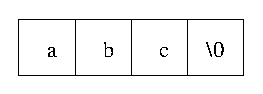
\includegraphics{1.eps}
\end{center}
\caption{Cadena en Memoria}
\end{figure}
********************* dejarla mejor *************

El car\'acter nulo ('$\backslash$0') se utliza en C para marcar el final de 
la cadena en memoria. Vamos a ver ahora un ejemplo de la utilizaci\'on de
las cadenas de caracteres.

\begin{quotation}
\begin{verbatim}

#include <stdio.h>
void main(void)
{
   printf("\nEl mundo es un vampiro"
	  " enviado para drenar.\n(%s)\n", "Billy Corgan");
}


\end{verbatim}
\end{quotation}

La salida del ejemplo es esta:

\begin{quotation}
\begin{verbatim}

El mundo es un vampiro enviado para drenar.
(Billy Corgan)

\end{verbatim}
\end{quotation}

En el ejemplo vemos que hay dos cosas nuevas; la divisi\'on de la cadena en 
dos l\'{\i}neas y el c\'odigo de formato \texttt{\%s}. Este c\'odigo le dice a
la funci\'on \texttt{printf} que escriba una cadena de caracteres en su lugar.
La otra novedad es que una cadena se puede escribir en varias l\'{\i}neas,
el compilador lo interpreta como una \'unica cadena siempre que se cierren las
comillas al final de la l\'{\i}nea y se abran en la siguiente. En C el final
de una instrucci\'on se detecta con un punto y coma.

Aqu\'{\i} hacemos una observaci\'on y es que \texttt{'x'} es distinto a
\texttt{"x"}.  La primera es una constante car\'acter que pertenece a un tipo
b\'asico (\texttt{char}).La segunda, \texttt{"x"} es una cadena de 
caracteres que contiene dos caracteres, \texttt{'x'} y 
\texttt{'$\backslash$0'}; por lo que es un vector compuesto por estos dos
caracteres. Vamos a hablar un poco m\'as sobre los vectores para tener una 
noci\'on b\'asica de ellos desde un principio. La forma de declarar una 
variable vector es:

\index{vector}

\begin{quotation}
\begin{verbatim}

tipo  variable[numero_de_elementos];

\end{verbatim}
\end{quotation}

y para acceder a cada elemento del vector

\begin{quotation}
\begin{verbatim}

variable[numero_de_elemento];

\end{verbatim}
\end{quotation}

Tiene que entenderse que el primer elemento de un vector  siempre va a ser el
n\'umero 0,

\begin{quotation}
\begin{verbatim}

variable[0];

\end{verbatim}
\end{quotation}

despu\'es el 1, 2, \ldots, as\'{\i} si declaramos 10 elementos, el primero 
ser\'a el 0, luego 2, hasta el \textbf{9}. \emph{No entrar\'{\i}a el 
n\'umero 10}. Vemos un ejemplo:

\begin{quotation}
\begin{verbatim}

#include <stdio.h>
void main(void)
{
   int x[2]; /*se reserva memoria para dos elementos tipo int*/
   x[0] = 12;
   x[1] = 7;
   /*x[2] no existe, no se ha reservado memoria para el*/
   printf("\nx[0] = %d\nx[1] = %d \n", x[0], x[1]);
}

\end{verbatim}
\end{quotation}

Si se hubiese dado un valor para \texttt{x[2]} normalmente se compila sin 
problemas, pero al ejecutar el programa \emph{el valor de esta variable se 
escribir\'a en una posici\'on de memoria no asignada}, pudiendo producir 
resultados inesperados como escribir sobre el c\'odigo del sistema operativo
u otro programa que est\'e en memoria en ese momento en el peor de los casos.
Esto es muy importante y hay que tener mucho cuidado.

\section{Operadores}

\index{operador}
\index{operando}

Un \emph{operador} es un s\'{\i}mbolo (suma, resta, divisi\'on, \ldots) 
que realiza una operaci\'on sobre sus operandos. Un \emph{operando} es
el dato (variable, n\'umero, vector, \ldots) que se manipula por el
operador. Los operadores de C se dividen en cuatro grupos.

\begin{enumerate}

\item Operadores aritm\'eticos.
\item Operadores relacionales y l\'ogicos.
\item Operadores a nivel de bits.
\item Operadores especiales.

\end{enumerate}

Definiremos tambi\'3n expresiones que contienen variables para producir 
nuevos valores.

\subsection{Operadores Aritm\'eticos}

\index{operador!aritm\'etico}

Como su nombre indica van a realizar operaciones aritm\'eticas. Los 
representamos en la tabla 2.5.

\begin{table}[!hbp]
\begin{tabular}{|c|l|}
\hline
\em Operador & \em Acci\'on\\\hline
\hline
-- & Resta, tambi\'en menos monario\\\hline
+ & Suma, tambi\'en mas monario\\\hline
* & Multiplicaci\'on\\\hline
/ & Divisi\'on\\\hline
\% & Divisi\'on de m\'odulo\\\hline
\texttt{--} & Decremento\\\hline
++ & Incremento\\\hline

\end{tabular}
\caption{Operadores Aritm\'eticos}
\end{table}

\index{incremento}
\index{decremento}

Los operadores de incremento y decremento s\'olo se pueden aplicar a variables,
no a constantes. El operador de incremento a\~nade 1 a su operando y el de
decremento resta 1. De otra forma, \texttt{++x} o \texttt{x++} es igual que
\texttt{x = x + 1} y de igual forma para el decremento.

Los operadores de incremento y decremento pueden ir delante o despu\'es del
operando. Si el operador \emph{precede} al operando, C lleva a cabo la 
operaci\'on \emph{antes de utilizar el valor del operando}. Si el operador
\emph{sigue} al operando, C utilizar\'a su valor \emph{antes de incrementarlo
o decrementarlo}. Otra definici\'on podr\'{\i}a ser: La expresi\'on 
\texttt{++x} incrementa a \texttt{x} \emph{antes} que su valor sea usado, 
mientras que \texttt{x++} la incrementa \emph{despu\'es} de que su valor ya
ha sido usado. Vamos a poner un ejemplo para que se comprenda mejor.

\begin{quotation}
\begin{verbatim}

int a, b;		int a, b;
a = 2;			a = 2;
b = ++a;		b = a++;

\end{verbatim}
\end{quotation}

En el primer ejemplo, al efectuarse la operaci\'on incremento, \texttt{a} tiene
el valor 3 y \texttt{b} el mismo. En el segundo, \texttt{a} tiene el valor 3
y ahora \texttt{b} tiene el valor 2. El incremento y decremento de operadores
s\'olo se puede aplicar a variables; una expresi\'on como \texttt{(i+j)++}
es ilegal.

Unos operadores tienen m\'as precedencia que otros al efectuarse operaciones,
esto es importante, ya que habr\'a que utilizar par\'entesis u otras 
acotaciones para no confundinos a la hora de platear operaciones entre los 
operandos, pudiendo llegar a cometer errores fatales. Solamente decir que
los operadores del mismo nivel de preferencia son evaluados por el compilador
de \emph{izquierda a derecha}. Se puede alterar el orden de evaluaci\'on con
el uso de par\'entesis.
La precedencia de los operadores aritm\'eticos al igual que la de los otros 
se muestra en una tabla de la p\'agina \pageref{precedencia}.

Vemos algunos ejemplos sobre la precedencia de estos operadores, se 
muestran en la tabla 2.6. Mirar la tabla de precedencias para ver el orden.

\begin{quotation}
\begin{verbatim}
x1 = 2 + 3 * 4			 x1 = 14
x2 = (2 + 3) * 4                 x2 = 20
x3 = -4 - (-1)                   x3 = -3
x4 = 10 / 2 % 3                  x4 = 2
x5 = ++x3 - x4                   x3 = -2; x5 = -4
x6 = x3++ - x4                   x6 = -4; x3 = -1
x1 = -x1                         x1 = -14
x2 = (x1 + x2) / x3              x2 = -6
x3 = ((x1++) + (x2++)) -x3       x3 = -19; x1 = -13; x2 = -5
x4 = -(-(-x3))                   x4 = 19
x5 = (x6 * x6 +x6 / x6)          x5 = 17
x6 = (x1++) + (++x2) - (++x6)    x2 = -4; x6 = -3; x2 = -14; x1 =-12
x1++                             x1 = -11
--x2                             x2 = -5
\end{verbatim}
\end{quotation}

\subsection{Operadores Relacionales y L\'ogicos}

\index{operador!relacional}
\index{operador!l\'ogico}

La palabra \emph{relacional} se refiere a la relaci\'on entre unos valores y
otros. La palabra \emph{l\'ogico} son las distintas formas en que esas 
relaciones pueden conectarse entre s\'{\i}. Los dos se basan en la idea de
verdadero y falso \footnote{true o false}. En C, cualquier valor distinto de
cero es cierto y si el valor es 0 es falso. Las expresiones que son ciertas
toman el valor 1 y las falsas el valor 0.

\begin{table}[!hbp]
\begin{tabular}{|c|l|c|l|}\hline
\em Operador & \em Acci\'on & \em Operador & \em Acci\'on\\\hline
\hline
$>$ & Mayor & \&\& & Y\\\hline
$>$= & Mayor o igual & \texttt{||} & O\\\hline
$<$ & Menor & ! & NO\\\hline
$<$= & Menor o igual\\\hline
== & Igual\\\hline
!= & No igual\\\hline

\end{tabular}
\caption{Operadores Relacionales y L\'ogicos}
\end{table}

\begin{table}[!hbp]
\begin{tabular}{|c|c|c|c|}\hline
p q & p \&\& q & p \texttt{||} q & !q\\\hline
0 0 & 0 & 0 & 1\\\hline
0 1 & 0 & 1 & 1\\\hline
1 0 & 1 & 1 & 0\\\hline
1 1 & 0 & 1 & 0\\\hline

\end{tabular}
\caption{Tabla de verdad para operadores l\'ogicos}
\end{table}

C tiene una particularidad que es que la evaluaci\'on de una expresi\'on acaba
cuando se sabe el resultado de dicha expresi\'on.

\begin{quotation}
\begin{verbatim}

0 && x
1 || x

\end{verbatim}
\end{quotation}

En las dos expresiones \textbf{no} se eval\'ua \texttt{x} al ser superfluo; en 
la primera expresi\'on al ser uno de los dos operandos 0, el otro no es 
necesario mirarlo, igual se puede decir de la segunda expresi\'on. Como los 
operadores \&\& y \texttt{||} se eval\'uan de izquierda a derecha, podemos 
decir que el segundo operando (el que contiene a la \texttt{x} no se eval\'ua.
Si la expresi\'on fuera \texttt{x \&\& 0} , se evaluar\'{\i} primero la 
\texttt{x} y se \'esta fuera cierta, se evaluar\'{\i}a el 0, y si la 
\texttt{x} fuera falsa no se eval\'ua el 0.

\subsection{Operadores a Nivel de Bits}

\index{operador!a nivel de bits}

Realizan operaciones los bits de un byte o una palabra\footnote{dos bytes}. 
S\'olo se pueden utilizar con los tipos \texttt{char} e \texttt{int}.

\begin{table}[!hbp]
\begin{tabular}{|c|l|}\hline
\em Operador & \em Acci\'on\\\hline
\hline
\& & Y\\\hline
\texttt{|} & O\\\hline
$\land$ & O exclusiva (XOR)\\\hline
$\sim$ & Complemento a uno (NOT)\\\hline
$>>$ & Desplazamiento a la derecha\\\hline
$<<$ & Desplazamiento a la izquierda\\\hline
\end{tabular}
\caption{Operadores a nivel de bits}
\end{table}

Las tablas de la verdad de los operadores \&, \texttt{|} y $\land$ son las 
mismas que las tablas de verdad para \&\&, \texttt{||} y ! respectivamente;
pero los operadores a nivel de bits trabajan bit a bit.

\begin{table}[!hbp]
\begin{tabular}{|c|c|}\hline
p q & p$\land$q\\\hline
\hline
0 0 & 0\\\hline
0 1 & 1\\\hline
1 0 & 1\\\hline
1 1 & 0\\\hline

\end{tabular}
\caption{Tabla de verdad para XOR}
\end{table}

Es significativo que los operadores relacionales y l\'ogicos producen siempre
un resultado que es 0 o 1, mientras que las operaciones a nivel de bits
producen \emph{cualquier valor arbitrario} de acuerdo con la operaci\'on
espec\'{\i}fica, puediendo dar valores distintos a 0 o 1. Por ejemplo:

\begin{itemize}

\item 2\&\&3 nos da un valor de 1. El compilador eval\'ua la exprexi\'on
1\&\&1 que es 1.

\item 2\&3 da un calor de 2. El compilador eval\'ua 00000010\&00000011 que es
00000010 (en decimal 2).

\end{itemize}

La sint\'axis para los operadores de desplazamiento es 

\begin{quotation}

expresi\'on $>>$ n\'umero de bits a desplazar a la derecha
expresi\'on $<<$ n\'umero de bits a desplazar a la izquierda

\end{quotation}

Hay que hacer dos observaciones sobre los operadores de desplazamiento.

\begin{enumerate}

\item Un desplazamiento no es una rotaci\'on. Es decir, los bits que salen
por un extreemo no se introducen por el otro.

\item A medida que se desplazan los bits hacia un extremo, se va rellenando
con ceros por el extremo opuesto. \textbf{Pero no en todos las computadoras
es as\'{\i}}. Si queremos introducir ceros y que el programa nos de 
portabilidad, lo tenemos que hacer expl\'{\i}citamente con una operaci\'on
and.

\end{enumerate}

\begin{description}

\item NOTA: Se deben hacer ejercicios relacionados con todos estos tipos de 
operadores para tener un dominio lo mayor posible sobre estos y comprenderlos
lo mejor posible. Se pueden encontrar problemas relacionados con los 
operadores en libros sobre matem\'atica.

\end{description}

\subsection{Operadores Especiales}

No entraremos en mayor detalle con estos operadores, se ver\'an a su tiempo
para evitar posibles confusiones que no vienen ahora a cuento. Los operadores
especiales son ? \& * sizeof , . -$>$ () \texttt{[]}.

\index{operador!condicional}

El \emph{operador codicional} ? tiene la forma general

\begin{quotation}
\begin{verbatim}

expresion1 ? expresion2 : expresion3

\end{verbatim}
\end{quotation}

donde los tres operandos son como su nombre indica expresiones de C. El 
operador ? act\'ua de esta forma: Se eval\'ua \texttt{expresion1}, si es 
cierta, eval\'ua  \texttt{expresion2} y toma su valor. Si \texttt{expresion1}
es falsa, eval\'ua \texttt{expresion3} y toma este valor para la expresi\'on.
Ejemplo:

\begin{quotation}
\begin{verbatim}

2 < 3 ? 4 : 5
2 > 3 ? 4 : 5
1 < 2 ? (4 > 3 ? 2 : 3) : 5

\end{verbatim}
\end{quotation}

La primera toma el valor 4, la segunda el valor 5 y la tercera el valor 2.

\index{operador!direcci\'on}
\index{operador!contenido}

Los operadores de \emph{direcci\'on} y \emph{contenido} (\& y *) operan con
punteros y son monarios. El sentido del operador * no tiene nada que ver con
el operador aritm\'etico *. No debe haber confusi\'on porque uno es monario
y otro binario. Lo mismo se puede decir del operador \&.

\index{operador!sizeof}

El operador \texttt{sizeof} es monario y toma la \emph{longitud}, en 
\emph{bytes}, de una expresi\'on o de un tipo; en este \'ultimo caso tiene que
estar entre par\'entesis.

\index{operador!coma}

El operador como tiene dos usos distintos en C.

\begin{enumerate}

\item Como operador.

\item Para representar una lista de elementos.

\end{enumerate}

\begin{quotation}
\begin{verbatim}

int a, b, c;

\end{verbatim}
\end{quotation}

Como operador la como encadena varias expresiones. Estas operaciones son
evaluadas de izquierda a derecha y el valor de la expresi\'on total es el
valor de la expresi\'on m\'as a la derecha.

\index{operador!punto}
\index{operador!flecha}

Los operadores \emph{punto} y \emph{flecha} se utilizan con dos tipos 
compuestos, \texttt{struc} y \texttt{union}. Se ver\'an m\'as adelante.

\index{operador!par\'entesis}

Los par\'entesis se pueden considerar como operadores que aumentan la 
precedencia de  las operaciones que contienen. Tambi\'en se utilizan para 
especificar la llamada a una funci\'on.

\index{operador!corchete}

Los corchetes llevan a cabo el indexamiento de vectores.

\section{Sentencias de Asignaci\'on}

Son sentencias de C en las que se asigna un valor a una variable. Su forma 
general es  \texttt{variable operador\_asignaci\'on expresi\'on}. Los 
operadores son estos:

\begin{quotation}
\begin{verbatim}

=  *=  /=  %=  +=  -=  <<=  >>=  &=  ^=  |=

\end{verbatim}
\end{quotation}

El significado del operador \texttt{=} es redundante. Las sentencias de 
asignaci\'on son expresiones. El valor de la expresi\'on es el valor que se
le asigna a la variable. Se eval\'uan de \emph{derecha a izquierda}, por
ejemplo.


\begin{quotation}
\begin{verbatim}

int a, b;
a = b = 3

\end{verbatim}
\end{quotation}


Primero se asigna el 2 a la \texttt{b} y despu\'es a la \texttt{a}. En la tabla
2.8 se exponen los dem\'as operadores de asignaci\'on.

\begin{table}[!hbp]
\begin{tabular}{|p{0.8in}|p{1.1in}|}\hline
\em Sentencia de asignaci\'on & \em Sentencia de asignaci\'on correspondiente\\
\hline
\hline
x *= y & x = x * y\\\hline
x /= y & x = x / y\\\hline
x \%= y & x = x \% y\\\hline
x += y & x = x + y\\\hline
x --= y & x = x -- y\\\hline
x $<<$= y & x = x $<<$ y\\\hline
x $>>$= y & x = x $>>$ y\\\hline
x \&= y & x = x \& y\\\hline
x $\land$= y & x = x $\land$ y\\\hline
x \texttt{|}= y & x = x \texttt{|} y\\\hline

\end{tabular}
\caption{Operadores de Asignaci\'on}
\end{table}

\section{Inicializaci\'on de Variables}

La forma de inicializar variables es:

\begin{quotation}
\begin{verbatim}

tipo variable = expresion;

\end{verbatim}
\end{quotation}

Ejemplo:

\begin{quotation}
\begin{verbatim}

double d = 12.3;

\end{verbatim}
\end{quotation}

Tambi\'en se pueden inicializar varias variables en la misma l\'{\i}nea
siempre que estas est\'en separadas por comas.

\begin{quotation}
\begin{verbatim}

char cadena, otra, d, a;

\end{verbatim}
\end{quotation}

\section{Conversi\'on de Tipos}

\index{conversi\'on}

La concersi\'on de tipos es algo importante que hay que tener en cuenta ya que
puede dar lugar a errores inesperados. Se refiere a la situaci\'on en que se
 mezclan variables de distinto tipo. Si esto ocurre en una  sentencia de 
asignaci\'on, la regla de conversi\'on es f\'acil: \emph{el valor del lado
derecho de la expresi\'on se convierte al del lado izquierdo}. Ejemplo:

\begin{quotation}
\begin{verbatim}

int a = 4.1; /*2.3 se convierte en 2*/
char ca = 233 /*los bits mas significativos de 233 se pierden*/

\end{verbatim}
\end{quotation}

El tipo que resulta de aplicar un operador con dos operandos de tipos
 diferentes es el tipo de mayor tama\~no, el de mayor logitud en bytes. 
Si hacemos la operaaci\'on 4 + 2.34 el valor de esta expresi\'on es 6.34,
un valor de tipo \texttt{float}.

Es posible forzar a que una expresi\'on sea de un tipo determinado con el uso
de una expresi\'on denominada \emph{molde}. La forma general es 
\texttt{(tipo) expresi\'on}. Es decir, poniendo entre par\'entesis el tipo
que queramos que prevalezca. El molde se puede considerar como un operador
\emph{monario} teniendo la misma precedencia que los dem\'as operadores 
monarios. Ejemplos:

\begin{table}[!hbp]
\begin{tabular}{c c c}

\em Expresi\'on & \em Valor de la expresi\'on & \em Tipo de la expresi\'on\\
3 / 2 & int & 1 \\
3.0 / 2 & float & 1.5\\
(float) 3 / 2 & float & 1.5\\
\end{tabular}
\end{table}

\section{Precedencia de los Operadores}

\label{precedencia}
\index{precedencia}

En la tabla 2.11

\begin{table}[!hbp]
\begin{tabular}{|l|c|}\hline
\em Operadores & \em Asociatividad\\\hline
\hline
() \texttt{[]} -$>$ . & de izquierda a derecha\\\hline
! $\sim$ ++ \texttt{--} + -- * \& (tipo) sizeof & de derecha a izquierda\\\hline
* / \% & de izquierda a derecha\\\hline
+ -- & de izquierda a derecha\\\hline
$<<$ $>>$ & de izquierda a derecha\\\hline
$<$ $<$= $>$ $>$= & de izquierda a derecha\\\hline
== != & de izquierda a derecha\\\hline
\& & de izquierda a derecha\\\hline
$\land$ & de izquierda a derecha\\\hline
\texttt{|} & de izquierda a derecha\\\hline
\&\& & de izquierda a derecha\\\hline
\texttt{||} & de izquierda a derecha\\\hline
?: & de derecha a izquierda\\\hline
= += --= *= /= \%= \&= $\land$= \texttt{|}= $<<$= $>>$= & de derecha a 
izquierda\\\hline
, & de izquierda a derecha\\\hline

\end{tabular}
\caption{Tabla de precedencias}
\end{table}

Los operadores unarios +, -- y * tienen mayor precedencia que sus formas 
binarias.

\section{Ejercicios}

\begin{itemize}

\item \textbf{Ejercicio 2--1.} Dada la funci\'on

$y = \frac{1}{4} x$

dise\~nar un programa que para el valor de la abcisa 4.4 de la 
correspondiente ordenada. La anterior expresi\'on en C se 
escribe de la forma:

y = (1.0 / 4) * x;
\'o
y = (1 / 4.0 ) * x;

ya que si se hace 1/4, el resultado ser\'a 0. Otras soluciones
son:

y = ((float) 1/4) * x;
\'o
y = (1 / (float) 4) * x;

\end{itemize}


\end{document}
